\documentclass{beamer}

\usepackage{default}

\usepackage[T2A]{fontenc}
\usepackage[utf8]{inputenc}
\usepackage[english,russian]{babel}

%\usepackage{mathptmx}% http://ctan.org/pkg/mathptmx

\usepackage{graphicx}
\usepackage{tabularx}
\usepackage{dcolumn}

\DeclareMathVersion{nxbold}
\SetSymbolFont{operators}{nxbold}{OT1}{cmr} {b}{n}
\SetSymbolFont{letters}  {nxbold}{OML}{cmm} {b}{it}
\SetSymbolFont{symbols}  {nxbold}{OMS}{cmsy}{b}{n}

\usepackage{amsfonts}
\usepackage{mathtools}

\usepackage{hyperref}
\usepackage{url}

\def\bbljan{Jan.}
\def\bblfeb{Feb.}
\def\bblmar{Mar.}
\def\bblapr{Apr.}
\def\bblmay{May}
\def\bbljun{Jun.}
\def\bbljul{Jul.}
\def\bblaug{Aug.}
\def\bblsep{Sep.}
\def\bbloct{Oct.}
\def\bblnov{Nov.}
\def\bbldec{Dec.}

% Добавим своих математических операторов
\DeclareMathOperator*{\argmin}{arg\,min}


%\usetheme{Warsaw}


\begin{document}

\title[Age progression] % (optional, only for long titles)
{Исследование методов определения и изменения возраста человека по фотографии}
\subtitle{Выпускная квалификационная работа}
\author % (optional, for multiple authors)
{Василихин~Ростислав}
\institute % (optional)
{
  Национальный исследовательский университет\\
  Высшая школа экономики
}
\date % (optional)
{Нижний Новгород, 2015}
\subject{Выпускная квалификационная работа}

\frame{\titlepage}
	
  \begin{frame}
  	\frametitle{Имитация возрастных изменений}
  	\begin{itemize}
	  	\item Поиск пропавших детей
	  	\item Распознавание лиц
	  	\item Обновление баз фотографий
  	\end{itemize}
  	\begin{figure}[t]
		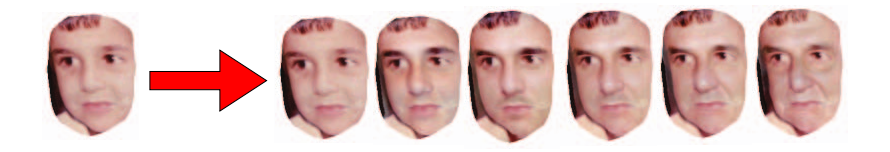
\includegraphics[width=\textwidth]{ilaware_slide.png}
	\end{figure}
	\begin{figure}[t]
		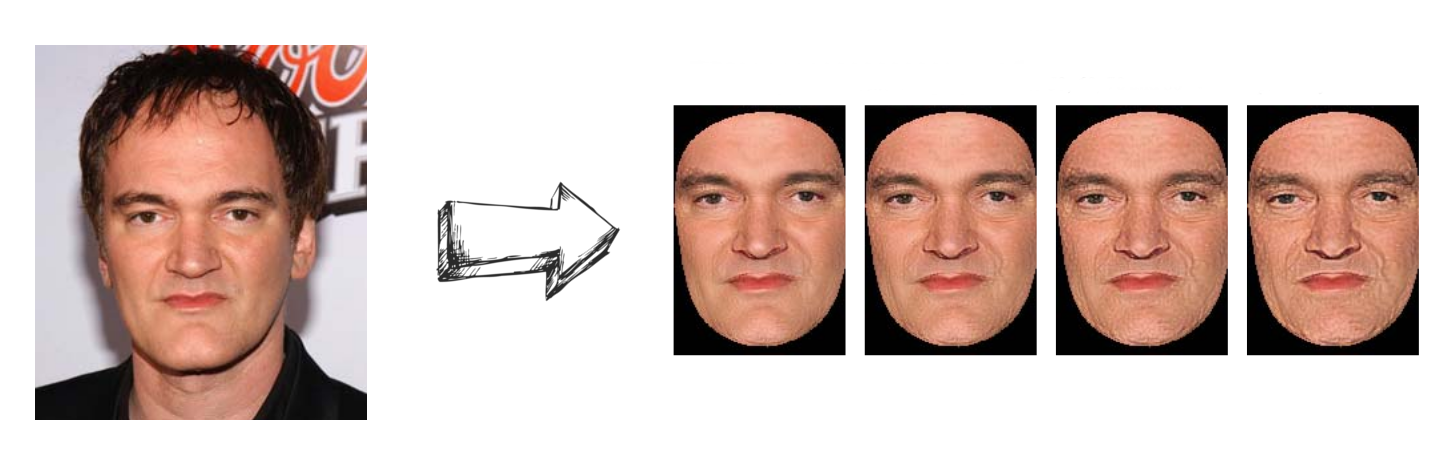
\includegraphics[width=\textwidth]{quentin.png}
	\end{figure}
  \end{frame}
	
  \begin{frame}
	\frametitle{Оценка возраста по фото}
	\begin{figure}
  		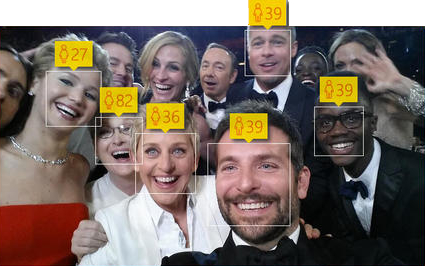
\includegraphics[width=0.5\textwidth,keepaspectratio]{how_old.jpeg}
	\end{figure}
	\begin{figure}
  		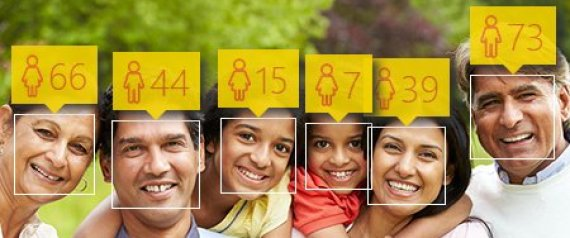
\includegraphics[width=0.5\textwidth,keepaspectratio]{how_old2.jpg}				
	\end{figure}
  \end{frame}
  
  \begin{frame}
    \frametitle{Задачи}
    \begin{enumerate}
		\item Исследовать популярные методы оценки возраста по фото
    		\item Исследовать популярные подходы к задаче имитации возраста
    		\item Реализовать ключевые компоненты системы имитации возраста
    \end{enumerate}
  \end{frame}
  
  \begin{frame}
  	\frametitle{Оценка возраста по фото}
  	\framesubtitle{Популярные методы}
  	%More content goes here
  	\begin{itemize}
  	\item Ранние методы:
  		\begin{itemize}
  			\item сегментация по цвету лица
  			\item анализ пропорций между отдельными частями лица
  			\item поиск морщин
  		\end{itemize}

	\vspace{1em}	

  	\item Maulin Gandhi, 2004:
		\begin{enumerate}
			\item ручная разметка		
			\item предобработка
			\item SVR
		\end{enumerate}
		
	\vspace{1em}	
	 	 	 
  	\item Eidinger, Hassner, 2014:
		\begin{enumerate}
  			\item поиск лица с помощью Viola-Jones, 2001
  			\item выравнивание по задетектированным ключевым точкам (Zhu-Ramanan, 2012)
  			\item dropout SVM
  		\end{enumerate}  	
  	\end{itemize}  	
  \end{frame}
  
  \begin{frame}
  	\frametitle{Оценка возраста по фото}
   	\framesubtitle{Age and Gender Classification Using CNN, 2015}
   	\begin{itemize}
   		\item Классификация на 8 возрастных групп
   		\item Искусственная нейронная сеть со свёрточными слоями
   		\item Не требуется предобработка
	\end{itemize}	
	\begin{figure}
		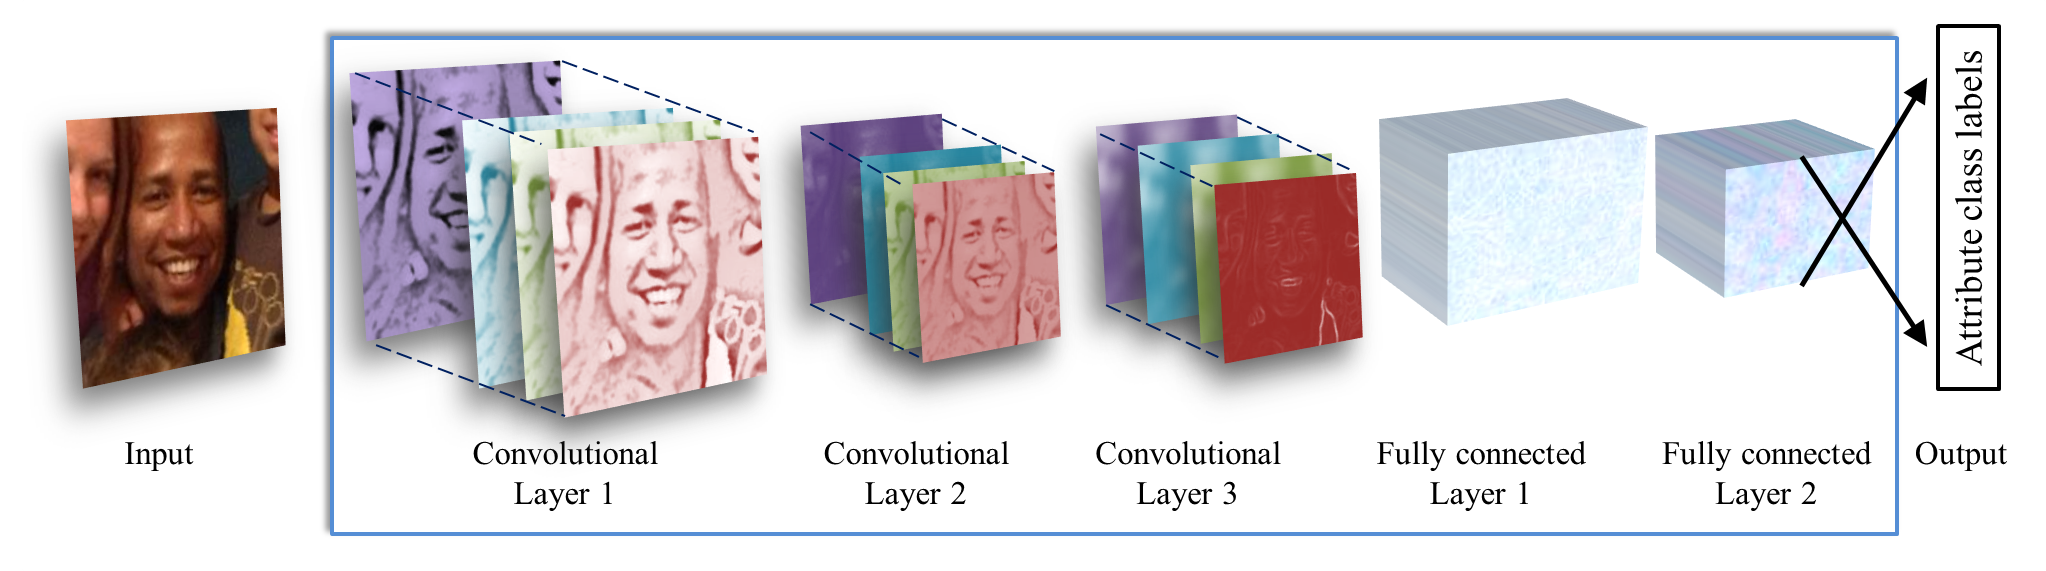
\includegraphics[width=\textwidth]{cnn.png}
	\end{figure}
  \end{frame}
    
  \begin{frame}
	  \frametitle{Оценка возраста по фото}
	  \framesubtitle{Эксперименты}
	  \begin{itemize}
	  	\item Age and Gender Classification Using CNN, 2015
	  	\item 3121 фотография из соцсетей
	  	\item Python, Caffe, Numpy
	  	\item Результаты:
	  	\begin{enumerate}
	  		\item в 45\% случаев класс угадан точно
	  		\item в 75\% случаев класс угадан с ошибкой $\leq1$  кластер
	  		\item средняя ошибка -4,39 лет
	  		\item средняя абсолютная ошибка 9,37 лет
	  		\item стандартное отклонение 14,72 лет
	  	\end{enumerate}
	  \end{itemize}
  \end{frame}   
  
  \begin{frame}
  	  \frametitle{Имитация возраста по фото}
  	  \framesubtitle{Популярные методы}
  	  \begin{itemize}
  	  	\item Ранние методы:
  	  	\begin{itemize}
  	  		\item методы, основанные на анатомии лица
  	  		\item активная модель формы для поиска ключевых точек
  	  		\item метод главных компонент для текстуры лица
  	  		\item оценка изменения параметров вейвлет-разложения
  	  	\end{itemize}

		\vspace{1em}	  	  	
  	  	
  	  	\item Maulin Gandhi, 2004:
		\begin{enumerate}
			\item предобработка и ручная разметка
			\item оценка возраста
			\item IBSDT: перенос нормалей с одного изображения на другое
		\end{enumerate}
  	  \end{itemize}
  	  \begin{figure}
  	  	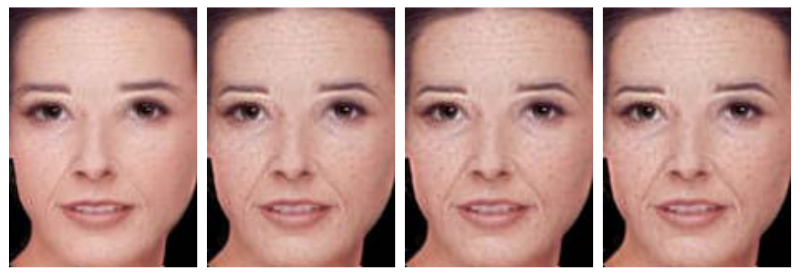
\includegraphics[width=\textwidth]{gandhi_slide.png}
  	  \end{figure}
  \end{frame}
  
  \begin{frame}
  	  \frametitle{Имитация возраста по фото}
  	  \framesubtitle{Illumination-Aware Age Progression, 2014}
  	  На вход поступает изображение лица, его исходный возраст и желаемый возраст
  	  \begin{enumerate}
  	  	\item Предобработка
  	  	\begin{itemize}
  	  		\item детектирование лица
  	  		\item выравнивание позы лица
  	  	\end{itemize}
  	  	\item Нейтрализация выражения лица
  	  	\item Поиск попиксельного соответствия (оптического потока) между лицами
  	  	\item Перенос освещённости со входного изображения на усреднённые образцы
  	  	\item Перенос текстурных изменений на исходное лицо
  	  	\item Перенос изменений в потоке на лицо
  	  \end{enumerate}
  \end{frame}
  
  \begin{frame}
	  \frametitle{Имитация возраста по фото}
	  \framesubtitle{Подзадачи}
	  Обучение:
	  \begin{enumerate}
	  	\item \textbf{Выравнивание изображений внутри каждого кластера}
	  	\item Вычисление relightable-моделей методом главных компонент
	  	\item Вычисление оптического потока между кластерами
	  \end{enumerate}	  	  
	  
	  \vspace{1em}	  
	  
	  Имитация возраста:
	  \begin{enumerate}
	  	\item \textbf{Получение текущего возраста по фото}
	  	\item \textbf{Выравнивание фото}
	  	\item Имитация текстурных изменений
	  	\item Имитация изменений в оптическом потоке
	  \end{enumerate}
	  
  \end{frame}
  
  \begin{frame}
  	  \frametitle{Методы выравнивания фото}
  	  \framesubtitle{Collection flow}
  	  Вычисляет попарный оптический поток между изображениями лиц из коллекции за $O(n)$ операций
	  \begin{enumerate}
	  	\item Метод главных компонент для коллекции изображений
	  	\item Проекция на подпространство главных компонент
	  	\item Вычисление оптического потока между проекцией и оригиналом
	  	\item Искривление оригинала оптическим потоком
	  	\item Итеративный подбор оптимального числа главных компонент
	  \end{enumerate}
  \end{frame}
  
  \begin{frame}
  	  \frametitle{Методы выравнивания фото}
   	  \framesubtitle{Искривление по ключевым точкам}
   	  \begin{columns}
	  	\begin{column}{0.5\textwidth}
	  		\begin{enumerate}
				\item Детектирование набора ключевых точек на лице
				\item Кадрирование лица по ключевым точкам
				\item Искривление изображения с целью выравнить позу лица
   	  		\end{enumerate}
	  	\end{column}   	  
   	  	\begin{column}{0.5\textwidth}
   	  		\begin{figure}
   	  			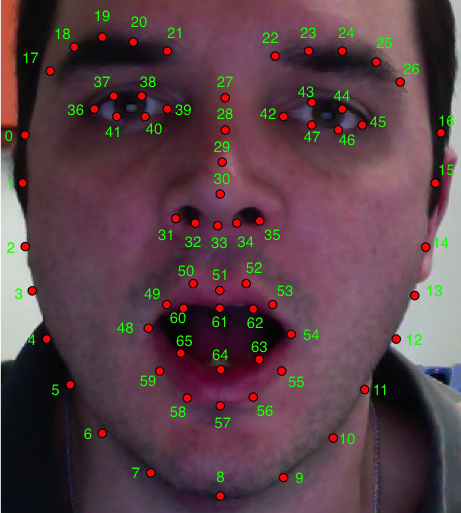
\includegraphics[width=\textwidth]{avatar-annotation.png}
   	    		\end{figure}
   	  	\end{column}
   	  \end{columns}
  \end{frame}
  
  \begin{frame}
  	  \frametitle{Методы выравнивания фото}
  	  \framesubtitle{Frontalization, 2015}
  	  Выравнивание позы лица с использованием 3d-модели и детектора ключевых точек
  	  \begin{enumerate}
  	  	\item Поиск ключевых точек на лице
  	  	\item Оценка позы головы по положению точек на 3d-модели
  	  	\item Обратная проекция изображения на 3d-модель в стандартной позе
  	  	\item Вычисление карты заслонений
  	  	\item Коррекция с использованием симметричной копии
  	  \end{enumerate}
  	  \begin{figure}
  	  	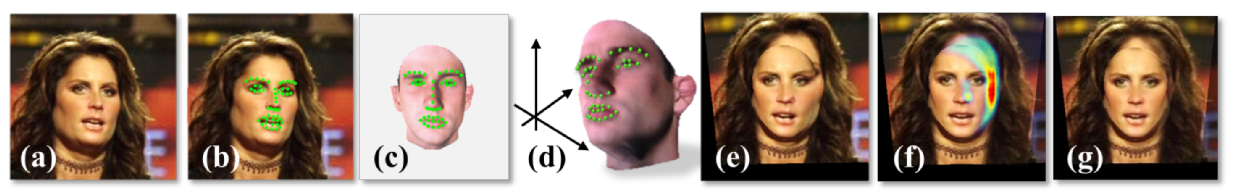
\includegraphics[width=\textwidth]{frontal2.png}
  	  \end{figure}
  \end{frame}
  
  \begin{frame}
  	  \frametitle{Методы выравнивания фото}
  	  \framesubtitle{Эксперименты}
	  \begin{itemize}
	  	\item Оценка качества выравнивания:
	  	\begin{itemize}
	  		\item Среднее изображение по выборке
	  		\item Средний модуль градиентов на среднем изображении
	  	\end{itemize}
	  	
	  	\vspace{1em}
		\item Выборка:
		\begin{itemize}
			\item 3121 фотография из соцсетей
			\item 309 фотографий одного и того же человека
        \end{itemize}
        
        \vspace{1em}
		\item Инструменты:
		\begin{itemize}
			\item С++
			\item OpenCV
		\end{itemize}				
	  \end{itemize}
  \end{frame}
  
  
  \begin{frame}
  	  \frametitle{Методы выравнивания фото}
  	  \framesubtitle{Эксперименты}
  	  Варианты:
	  \begin{itemize}
	  	\item \textbf{Без выравнивания}
	  	\item Collection flow
		\item Frontalization + детектор точек Saragih, 2010
		\item \textbf{Frontalization + детектор точек Zhu Ramanan, 2012}
		\item Искривление по ключевым точкам
		\item Все варианты Collection flow и Frontalization
	  \end{itemize}
	  \begin{figure}
	  	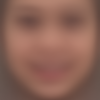
\includegraphics[width=0.2\textwidth]{results/all_no_mean.png}
	  	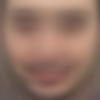
\includegraphics[width=0.2\textwidth]{results/id2_no_mean.png}
	  	\hspace{1.5em}
	  	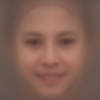
\includegraphics[width=0.2\textwidth]{results/all_front_mean.png}
	  	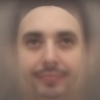
\includegraphics[width=0.2\textwidth]{results/id2_front_mean.png}
	  \end{figure}
  \end{frame}
  
 
  \begin{frame}
  	  \frametitle{Заключение}
  	  \begin{itemize}
  	  	\item Исследованы алгоритмы детектирования возраста
  	  	\item Проведены эксперименты и собрана статистика по одному из них
		\item Исследованы популярные алгоритмы имитации возраста
		\item Реализованы наиболее важные из компонентов этого алгоритма
  	  \end{itemize}
  \end{frame}
  
  \begin{frame}
  	  \begin{center}
  	  Спасибо за внимание!
  	  \end{center}
  \end{frame}
  
\end{document}
